\documentclass[border=5mm]{standalone}
\usepackage{tikz}
\usetikzlibrary{calc, arrows.meta, decorations.markings}

\begin{document}
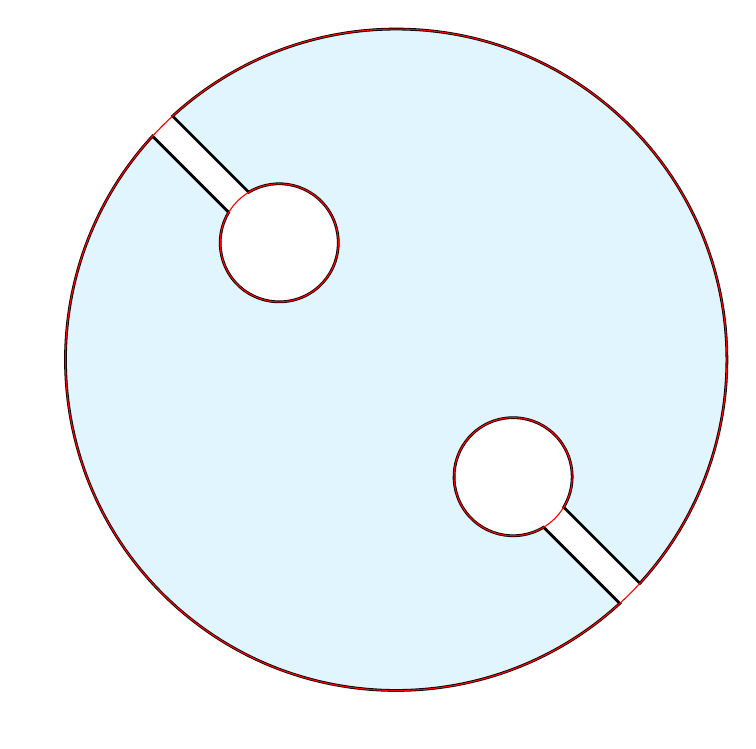
\begin{tikzpicture}[>=Latex, scale=1.5]
    \def\R{2.8}
    \def\r{0.5}
    \def\delta{0.12}

    \pgfmathsetmacro{\aOut}{asin(\delta/\R)}
    \pgfmathsetmacro{\aIn}{asin(\delta/\r)}

    % Z1 at 135
    \coordinate (Z1) at (135:1.4);
    % Z2 at 315
    \coordinate (Z2) at (315:1.4);

    \draw[cyan!12, fill=cyan!12, draw=black, line width=1pt]
        (0:\R) arc (0:135-\aOut:\R)
        -- ($ (Z1) + (135-\aIn:\r) $)
        arc (135-\aIn : -225+\aIn : \r)
        -- (135+\aOut:\R)
        arc (135+\aOut : 315-\aOut : \R)
        -- ($ (Z2) + (315-\aIn:\r) $)
        arc (315-\aIn : -45+\aIn : \r)
        -- (315+\aOut:\R)
        arc (315+\aOut : 360:\R) -- cycle;

    \draw[red] (0,0) circle (\R);
    \draw[red] (Z1) circle (\r);
    \draw[red] (Z2) circle (\r);
\end{tikzpicture}
\end{document}
